\section{Arhitektura sistema}

Karakteristike arhitekture informacionog sistema:

\textbf{Tip aplikacija}
\begin{itemize}
\item desktop aplikacija
\end{itemize}

\textbf{Strategije isporučivanja}
\begin{itemize}
\item Baza podataka na serveru postavljena
\begin{enumerate}
\item aplikacija na klijentski kompjuterima
\item aplikacija na jakom serveru, koji ima više korisnika (remote desktop pristup)
\end{enumerate}
\end{itemize}

\textbf{Tehnologije:}
\begin{itemize}
\item Java, JavaFX , MySQL
\end{itemize}

\textbf{Kriterijumi prihvatljivosti:}
\begin{itemize}
\item Jednostavnost u primeni, radi brzog prelaženja na novi sistem sa starog
\end{itemize}

\textbf{Popratne komponente:}
\begin{itemize}
\item Autentifikacija (korisnički nalog vezan sa korisničkim nalog baze podataka)
\item Pravljenje kopija baze podataka
\item Dokumentacija
\end{itemize}

\clearpage

\begin{figure}[ht]
\centering
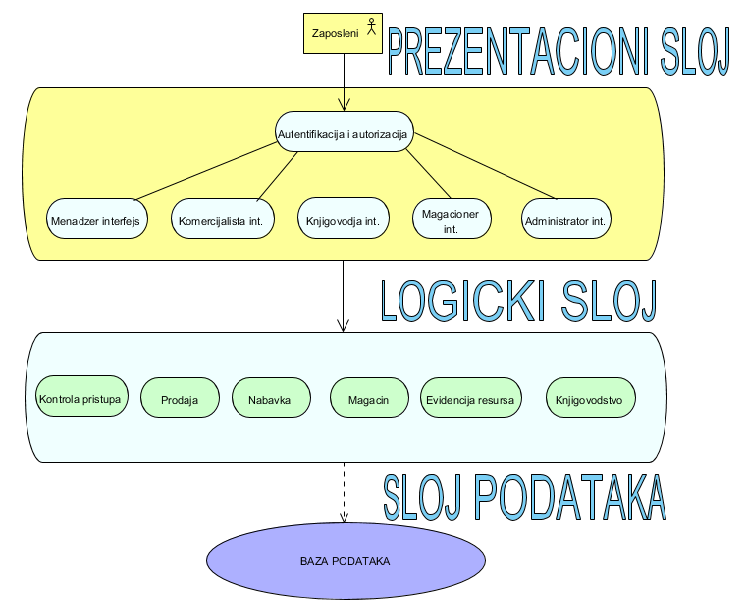
\includegraphics[width=165mm]{slike/Arhitektura.png}%
\caption{Arhitektura sistema}
\end{figure}

\subsection{Tip arhitekture}

Arhitektura ovih aplikacija je klijent-server arhitektura. Sastoji se od prezentacionog sloja,
logičkog sloja na klijentskoj strani, dok se sloj podataka nalazi na serveru.

[Alternativno: server deli na više korisnika koji imaju aplikacije (remote desktop pristup), dok im je baza podataka zajednička]

\subsubsection{Prezentacioni sloj}

Vizuelna reprezentacija
informacionog sistema. Nakon prijavljivanja korisnika na sistem, u zavisnosti od položaja u firmi pojavljuju mu se oblasti za koje je zadužen i fukncije koje može obavljati.

\subsubsection{Logički sloj}

Logički sloj je podeljen na više sektora i obezbeđuje logičku podršku prezentacionom
sloju, takođe obezbeđuje komunikaciju sa bazom.

\textbf{Kontrola pristupa:}
Bavi se autentifikacijom i autorizacijom korisnika programa.

\textbf{Prodaja:}
Prodaja zadužena za dokumente porudžbine, ponude, otpremnice, fakture. Operacije čitanja, izmene, brisanje i kreiranje novih dokumenata.

\textbf{Nabavka:}
Nabavka zadužena za dokumente narudžbine, ponude, prijemnice, fakture. Operacije čitanja, izmene, brisanje i kreiranje novih dokumenata.

\textbf{Magacin:}
Magacin zadužena za dokumente prijemnice, otpremnice, popise. Operacije čitanja, izmene, brisanje i kreiranje novih dokumenata.

\textbf{Knjigovodstvo:}
Knjigovodstvo zadužena za dokumente ulaznih i izlaznih faktura, kao i evidentiranje popisa. Obrada zarada, poreza i troškova.

\textbf{Evidencija resursa:}
Ažuriranje i unos novih zaposlenih, proizvoda i ostalih resura firme.

\subsubsection{Sloj podataka}

Sloj podataka sadrži bazu podataka koja se nalazi na jedinstvenom serveru, koriste je sve klijentske aplikacije.

\clearpage

\section{Zaključak}

Informacioni sistem veleprodaje je osnovni deo poslovanja firmu koje se bave trgovinom u raznim oblastima.

Ciljevi su sistematsko i transparentno čuvanje dokumenata, kako bi sve bilo u skladu sa zakonima poslovanja. 

Nadamo se da bi ovaj sistem mogao u stvarnosti da se implementira i bude funkcionalan, uz obevezna prilagodjavanja konretnom poslovanju.

Mislili smo da je imlementacija najbitniji deo, medjutim detaljno planiranje sistema je bar podjednako važno, ako ne i važnije.




